\documentclass{article}

\usepackage{graphicx}
\usepackage{tikz}
\usepackage{tikzsymbols}
\usetikzlibrary{calc,patterns,shapes.geometric}
\pagestyle{empty}
\usepackage[margin=0pt]{geometry}
\geometry{papersize={14in,12in}}

\def\centerarc[#1](#2)(#3:#4:#5){\draw[#1] ($(#2)+({#5*cos(#3)},{#5*sin(#3)})$) arc (#3:#4:#5);}

\begin{document}
	\begin{figure}
		\centering
		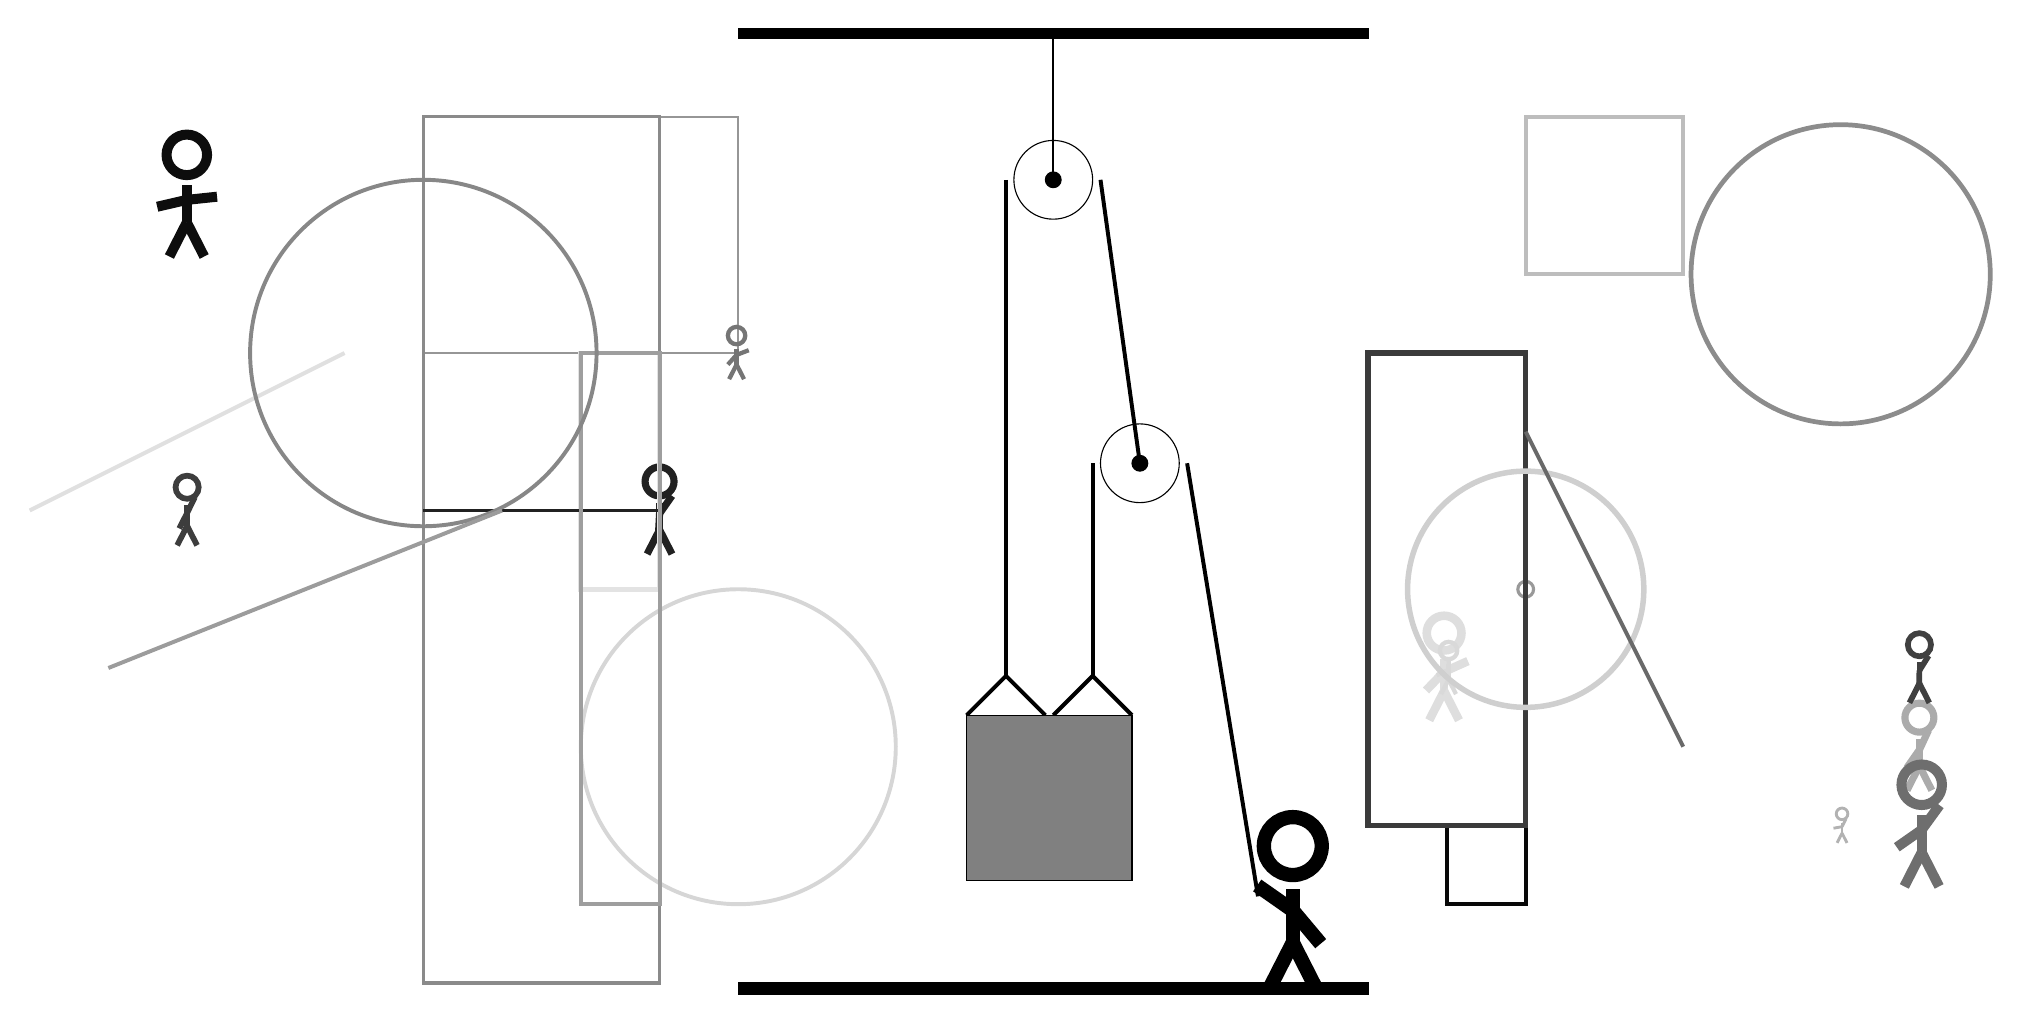
\begin{tikzpicture}
			%%%%% START %%%%%
			
			\draw[fill=black] (-2, 9) rectangle (6, 9.125);
			
			\draw (2, 7.2) circle (0.5);
			\draw[fill=black] (2, 7.2) circle (0.1);
			\draw[thick] (2, 7.2) -- (2, 9);
			
			\draw (3.1, 3.6) circle (0.5);
			\draw[fill=black] (3.1, 3.6) circle (0.1);
			
			\draw[line width = 0.5mm]  (0.9, 0.4) -- (1.4, 0.9) -- (1.9, 0.4);
			\draw[line width = 0.5mm]  (2.0, 0.4) -- (2.5, 0.9) -- (3.0, 0.4);
			\draw[fill=black!50] (0.9, 0.4) rectangle (3.0, -1.7);
			
			\draw[line width = 0.5mm] (1.4, 7.2) -- (1.4, 0.9);
			\centerarc[line width = 0.5mm](2, 7.2)(0:180:0.6);
			\draw[line width = 0.5mm] (2.6, 7.2) -- (3.1, 3.6);
			\draw[line width = 0.5mm] (2.5, 3.6) -- (2.5, 0.9);
			\centerarc[line width = 0.5mm](3.1, 3.6)(0:180:0.6);
			\draw[line width = 0.5mm] (3.7, 3.6) -- (4.6, -1.9);
			
			\node at (5, -2) {\Strichmaxerl[10][-35][-50]};
			
			\draw[line width=0.5mm, color=black!26] (8, 8) rectangle (10, 6);
			
			\node[line width=0.7mm, color=black!33] at (13, 0) {\Strichmaxerl[5][55][65]};
			\node[line width=0.5mm, color=black!87] at (-3, 3) {\Strichmaxerl[5][87][55]};
			\node[line width=0.3mm, color=black!13] at (7, 1) {\Strichmaxerl[6][46][24]};
			
			\node[line width=0.5mm, color=black!76] at (-9, 3) {\Strichmaxerl[4][63][64]};
			\draw [line width=0.5mm, color=black!16](-2, 0) circle (2.0);
			
			\draw [line width=0.4mm, color=black!40](8, 2) circle (0.1);
			
			\draw[line width=0.5mm, color=black!12](-7, 5) -- (-11, 3);
			\draw[line width=0.3mm, color=black!41] (-2, 5) rectangle (-6, 8);
			
			\draw[line width=0.4mm, color=black!46] (-3, 8) rectangle (-6, -3);
			\node[line width=0.7mm, color=black!57] at (13, -1) {\Strichmaxerl[7][35][54]};
			\draw[line width=0.5mm, color=black!97] (8, -1) rectangle (7, -2);
			\node[line width=0.6mm, color=black!15] at (7, 1) {\Strichmaxerl[3][24][89]};
			
			\draw[line width=0.6mm, color=black!11] (-3, 2) rectangle (-4, 5);
			\draw[line width=0.5mm, color=black!87](-3, 3) -- (-6, 3);
			\draw[line width=0.5mm, color=black!38] (-3, -2) rectangle (-4, 5);
			
			\draw [line width=0.6mm, color=black!45](12, 6) circle (1.9);
			\draw [line width=0.5mm, color=black!47](-6, 5) circle (2.2);
			\node[line width=0.5mm, color=black!95] at (-9, 7) {\Strichmaxerl[7][13][6]};
			
			\draw[line width=0.7mm, color=black!77] (6, -1) rectangle (8, 5);
			\draw[line width=0.5mm, color=black!39](-5, 3) -- (-10, 1);
			
			\node[line width=0.7mm, color=black!75] at (13, 1) {\Strichmaxerl[4][89][58]};
			
			\draw [line width=0.7mm, color=black!19](8, 2) circle (1.5);
			\node[line width=0.3mm, color=black!54] at (-2, 5) {\Strichmaxerl[3][48][21]};
			\node[line width=0.4mm, color=black!30] at (12, -1) {\Strichmaxerl[2][10][63]};
			\draw[line width=0.5mm, color=black!59](8, 4) -- (10, 0);
			
			
			\draw[fill=black] (-2, -3) rectangle (6, -3.15);
			
			%%%%% END %%%%%
		\end{tikzpicture}
	\end{figure}	
\end{document}